\documentclass{article}

\usepackage[margin=1in]{geometry}
\usepackage{minted}
\usepackage{amsmath}
\usepackage{amssymb}
\usepackage{graphicx}
\usepackage{subcaption}
%\usepackage{float}
\usepackage{xcolor}
\usepackage{setspace}
\usepackage{hyperref}
\usepackage[backend=biber]{biblatex}

\bibliography{progress-report.bib}
\doublespacing

\title{Final Project Progress Report}
\author{Leanna Calla\\Michael Stergianis}
\date{\today}

\begin{document}
\maketitle
\section{Interpolation}
\label{sec:interpolation}
Much of work in super resolution has to do with interpolation.  There
are many interpolation schemes that can be used in order to increase
the resolution of images. This section will briefly describe a few
interpolation schemes of note.
%
\subsection{Bilinear Interpolation}
\label{subsec:bilinear}
Bilinear interpolation is the process of supposing a subpixel
surrounded by four real pixels and interpolating linearly between the
four pixels to find the subpixel.
%
%
\section{Uses}
\label{sec:uses}

Super resolution is incredibly useful. As noted in
\cite{Yang2010ImageSH}, there are four main areas where super
resolution particularly useful.
\subsection{Surveillance Video}
As noted in \cite{Yang2010ImageSH}, super resolution has applications
when in the manipulations of surveillance videos. A video maybe frozen
to zoom into a specific area. This may help to look at things like faces or license plates.
\subsection{Remote Sensing}
\cite{Li} discusses the applications of super resolution on satellite
images. The figures below give an example of the improvements that can
be seen by applying a Wiener filter to a low resolution image. These
figures come from \cite{Li}.    
\begin{figure}[H]
  \centering
  \begin{subfigure}[b]{0.5\textwidth}
    \centering
  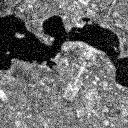
\includegraphics[width= 0.4\linewidth]{LR-satellite.png}
  \caption{\label{fig:label} Satellite low res }
\end{subfigure}%
\begin{subfigure}[b]{0.5\textwidth}
  \centering
  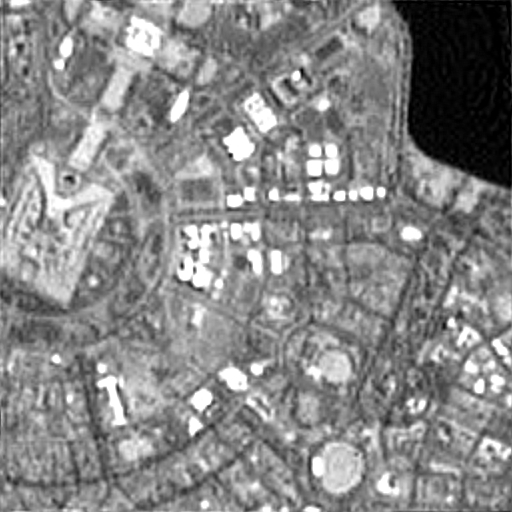
\includegraphics[width = 0.4\linewidth]{SR-satellite.png}
  \caption{\label{fig:label} Satellite super res }
  \end{subfigure}
\end{figure}


\subsection{Medical Imaging}
Super resolution has applications in Medical Imaging such as improving
the quality of MRI images. \cite{Peled} notes that the quality of the resolution of
an MRI is limited has limitations such as the imaging time and any
movement of the patient. The diffusion-sensitized echo-planar imaging
technique is acquires the image in shot, avoiding phase problems. Some
limitations do remain for brain images.  

\subsection{Video Standard Conversion}

\subsection{Multiple Image Resolution}
Low resolution images can be combined into one higher resolution
image. This is known as multiple image super resolution. In
\cite{CapelMulti}, we see that multiple images are used as training
data. This paper explores the use of training images
to set the constraints in the maximum likelihood estimation. Work is done of images of faces in \cite{CapelMulti}.
 
\section{Future Work}
\label{sec:future}
Hello world
%
\newpage
% Bibliography
\printbibliography
\end{document}
